%% --> Paquetes comunes
\usepackage{listings}
\usepackage{enumitem}
\usepackage{lipsum}
\usepackage{booktabs}
\usepackage{todonotes}
\usepackage[spanish,onelanguage,vlined,linesnumbered]{algorithm2e}
\setuptodonotes{color=colordef!50, size=\footnotesize}
\newcommand{\porhacer}[1]{\todo[inline]{\textbf{Por hacer:} #1}}

%% --> Definición de colores
\definecolor{codegreen}{HTML}{A5BE00}
\definecolor{codegray}{rgb}{0.5,0.5,0.5}
\definecolor{codepurple}{rgb}{0.58,0,0.82}
\definecolor{backcolour}{rgb}{0.95,0.95,0.92}

%% --> Estilo para código
\lstdefinestyle{mystyle}{
    language={[LaTeX]TeX}, % lenguaje
    basicstyle=\bfseries\ttfamily,
    keywordstyle=\color{colordef},
    commentstyle=\color{codegreen},
    % numbers=l,
    inputencoding=utf8,
    numberstyle=\color{gray},
    % numbers=left,
    xleftmargin=15pt,
    % backgroundcolor=\color{gray!15},
    showstringspaces=false,
    flexiblecolumns=true,
    stringstyle=\ttfamily\color{blue},
    extendedchars=true,
    emph={rm,bf,it,sf}, %...
    literate=%
    *{$}{{{\color{red}\$}}}1 % produce $ en rojo
    {$$}{{{\color{red}\$\$}}}1
    {ó}{{\'o}}1%
    {í}{{\'i}}1%
    {á}{{\'a}}1%
    {ú}{{\'u}}1%
}

%% --> Selección de estilo para el código
\lstset{
    style=mystyle,escapeinside={(*@}{@*)}
}

% Blancos tipográficos
\newcommand{\mq}{\hspace{0.5em}}  %medio cuadratín
\newcommand{\tq}{\hspace{0.33em}} % un terio de cuadratín
\newcommand{\qq}{\hspace{0.25em}} % un cuarto de cuadratín
\newcommand{\fs}{\hspace{0.125em}} % un octavo de cuadratín
\newcommand{\ep}{\hspace{0.05em}} % espacio de pelo

%% --> Nota para el material
\newcommand{\informacion}{\noindent\footnotesize{\color{colordef}
El presente material fue desarrollado por:

\noindent
\textbf{Daniel Lara}

\emph{Facultad de Ciencias, Escuela Politécnica Nacional}

\noindent
\textbf{Andrés Merino}

\emph{Facultad de Ciencias Exactas y Naturales, Pontificia Universidad Católica del Ecuador}


\medskip\noindent
La versión actual del material es 1.2-(Mayo 2021). En caso de encontrar inconsistencias o errores en el presente material se pueden comunicar a \href{mailto:daniel.lara@alephsub0.org}{daniel.lara@alephsub0.org}. Para más información puedes visitar nuestro sitio web: \href{https://alephsub0.org}{alephsub0.org}

\medskip\noindent

\includegraphics[height=12pt]{Imagenes/CreativeCommos/cc.eps} 
\includegraphics[height=12pt]{Imagenes/CreativeCommos/by.eps}
\includegraphics[height=12pt]{Imagenes/CreativeCommos/nc.eps}
\begin{minipage}[c]{0.85\textwidth}Esta obra se encuentra bajo licencia Atribución-NoComercial-CompartirIgual 4.0 Internacional (CC BY-NC-SA 4.0) Para más información puede visitar: \url{https://creativecommons.org/licenses/by-nc-sa/4.0/}\end{minipage}

\medskip\noindent
Si deseas colaborar con el desarrollo de este material, el código fuente está disponible en:   
\url{https://github.com/alephsub0/LaTeX_Guias.git}. Cualquier aporte (\emph{Pull request}) será de gran ayuda para mejorar este material. 

%% -- > Aquí se incluyen los nombres de los colaborades de estas guias:
% \medskip\noindent
% Otros colaboradores: Katheryn Yánes
}}

%%--> Formato para títulos
\titleformat{name=\section,numberless}[display]
  {\vspace*{-2mm}\bfseries\scshape\centering}
    {}{1ex}
    {\color{colortext}\large\titlerule\vspace{.05ex}
     }
    [\color{colortext}\vspace{.2ex}\titlerule]

\titleformat{\subsubsection}
    {\color{colortext}\normalsize\bfseries}
    {\thesubsubsection}{1em}{}
    
%% --> Datos de las guias
\universidad{Curso de \LaTeX}
\autor{Proyecto Alephsub0}
\materia{Introducción a \LaTeX}

%% --> Logos de las guias
\logouno[4.5cm]{Imagenes/Logos/LogoAlephsub0-02.eps}
\longtitulo{0.6\linewidth}
\fecha{Abril de 2021}

%% --> Nuevos ambientes
% \definecolor{coloryt}{rgb}{0.769,0.188,0.169}
%% Ambiente para enlaces de YouTube
\definecolor{coloryt}{HTML}{FF0000}
\newtcolorbox{ytcodigo}
    {icono=\faYoutubePlay,color=coloryt,postit}
%% Ambiente para código LaTeX  
\definecolor{colcod}{RGB}{174,218,255}
\newtcolorbox{ltcodigo}
    {icono=\faCode,color=colcod,postit,top=-2mm,bottom=-2mm}